%! TEX root = ./main.tex

\section{Kinematics}
\subsection{Rigid Body Kinematics}
\begin{minipage}[b]{0.43\linewidth}
    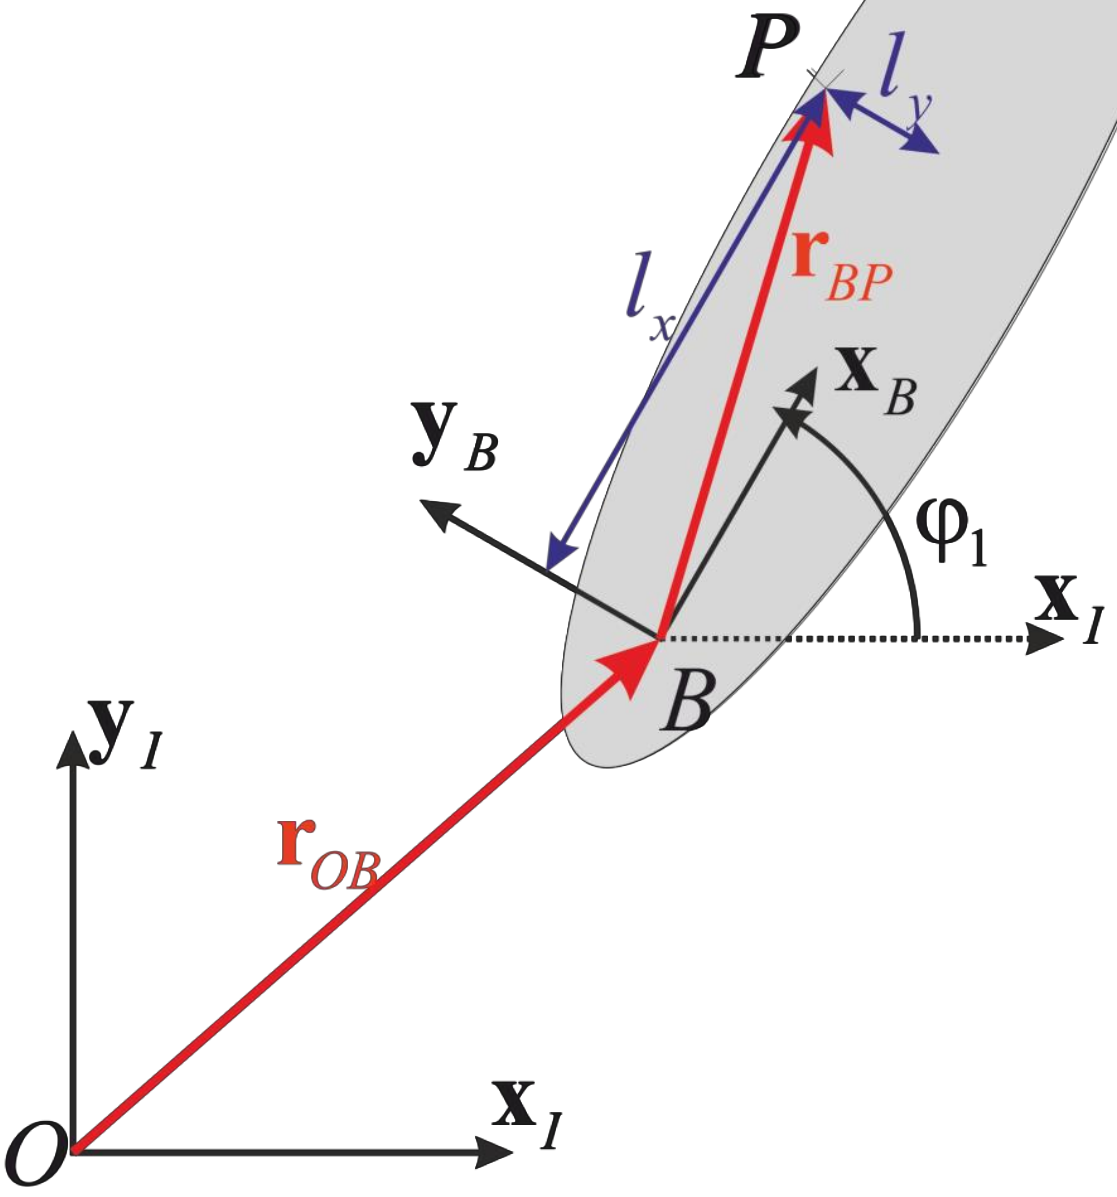
\includegraphics[width=\linewidth]{./Figures/03_RigidBodyTransformation.png}
\end{minipage}
\begin{minipage}[b]{0.55\linewidth}
    \raggedright
    \begin{itemize}
        \ides{Translation:} All pts of the body move parallele
            \begin{itemize}
                \item Vector from $O$ to $P$ in $I$: ${}_I r_{OP} = {}_I r_{OB} + {}_I r_{BP}$
                \item Velocity of of pt $P$ in $I$: ${}_I v_P = {}_I \dot r_{OP}$
            \end{itemize}
    \end{itemize}
\end{minipage}
\begin{itemize}
        \ides{Rotation:} One pt is fixed an all other move around it
            \begin{itemize}
                \item Vector $r$ in $B$ rotated to $I$: ${}_I r = R_{IB} {}_B r$
                \item Rotation $R_{IB}$ along $x, y, z$:
                    $\begin{bmatrix}
                        1 & 0 & 0\\
                        0 & \cos(\varphi) & -\sin(\varphi)\\
                        0 & \sin(\varphi) & \cos(\varphi)
                    \end{bmatrix}$
                    $\begin{bmatrix}
                        \cos(\varphi) & 0 & \sin(\varphi)\\
                        0 & 1 & 0\\
                        - \sin(\varphi) & 0 & \cos(\varphi)\\
                    \end{bmatrix}$
                    $\begin{bmatrix}
                        \cos(\varphi) & -\sin(\varphi) & 0\\
                        \sin(\varphi) & \cos(\varphi) & 0\\
                        0 & 0 & 1
                    \end{bmatrix}$
                \ides{Inverse:} $R_{BI} = R^{-1}_{IB} = R^\transpose_{IB}$
            \ides{Composition:} $R_{AI} = R_{AB} \cdot R_{BI}$
            \item Angular velocity of $B$ in $I$ along $z$: ${}_I \omega_{IB} = (0, 0, \dot \varphi)^\transpose$
                \begin{itemize}
                    \item Equal for every point in the body
                \end{itemize}
            \ides{Transformation:} ${}_I \omega_{IB} = R_{IB} \ {}_B \omega_{IB}$
            \ides{Composition:} ${}_I \omega_{IC} = {}_I \omega_{IB} + {}_I \omega_{BC}$
            \item ${}_I \hat \omega_{IB} = \dot R_{IB} R^\transpose_{IB} =
                \begin{bmatrix}
                    0 & -{}_I \omega^z_{IB} & {}_I \omega^y_{IB}\\
                    {}_I \omega^z_{IB} & 0 & -{}_I \omega^x_{IB}\\
                    -{}_I \omega^y_{IB} & {}_I \omega^x_{IB} & 0
                \end{bmatrix}, {}_I \omega_{IB} =
                \begin{bmatrix}
                    {}_I \omega^x_{IB}\\
                    {}_I \omega^y_{IB}\\
                    {}_I \omega^z_{IB}
                \end{bmatrix}$
        \end{itemize}
    \ides{Homogeneous Transformation:} Rotation $+$ Translation
        \begin{itemize}
            \item Vector from $O$ to $P$ in $I$: ${}_I r_{OP} = {}_I r_{OP} + R_{IB} \ {}_B r_{BP}$
            \item $
                \begin{pmatrix}
                    {}_I r_{OP}\\
                    1
                \end{pmatrix} =
                \begin{bmatrix}
                    R_{IB} & {}_I r_{OB}\\
                    0 & 1
                \end{bmatrix}
                \begin{pmatrix}
                    {}_B r_{BP}\\
                    1
                \end{pmatrix}$
            \item Full motion: ${}_I v_P = {}_I \dot r_{OP} = {}_I \dot r_{OB} + {}_I \omega_{IB} \times {}_I r_{BP}$
        \end{itemize}
    \ides{Vector Differentiation}
        \begin{itemize}
            \ides{Non-moving system:} ${}_I r \implies {}_I \dot r = \frac{d {}_I r}{dt}$
            \ides{Moving (translating or rotating) system:} ${}_B r \implies {}_B \dot r = \frac{d {}_B r}{dt} + {}_B \omega_{IB} \times {}_B r$
        \end{itemize}
    \ides{Generalized Coordinated}
        \begin{itemize}
            \item Set of independent variables that uniquely describe the robot's configuration
            \item $q = (q_1, q_2, \dots q_n)^\transpose$
            \item ${}_I r_{OP} = {}_I r_{OP}(q)$
        \end{itemize}
    \ides{Jacobians}
        \begin{itemize}
            \item $J_P = \frac{\partial r_{OP}(q)}{\partial q} =
                \begin{bmatrix}
                    \frac{\partial r_1}{\partial q_1} & \dots & \frac{\partial r_1}{\partial q_n}\\
                    \vdots & \ddots & \vdots\\
                    \frac{\partial r_m}{\partial q_1} & \dots & \frac{\partial r_1}{\partial q_n}\\
                \end{bmatrix}$
            \item Cartesian velocity to generalized velocity: $\dot r_P = J \dot q$
            \item Change in generalized coordinates to Cartesian space: $\bigtriangleup r_P = J \bigtriangleup q$
        \end{itemize}
\end{itemize}

\subsection{Inverse Kinematics}
\begin{itemize}
    \item Given desired endeffector position $r_{OF}(q) = r^{\text{goal}}_{OF}$, determine generalized coordinates $q$
    \item $r_{OF}(q)$ not easily invertible
\end{itemize}
\begin{minipage}[b]{0.6\linewidth}
    \begin{itemize}
        \ides{Iterative Method:}
            \begin{itemize}
                \item[1)] Initialize $q = q^0$ to initial guess and set $r = r(q)$
                \item[2)] Evaluate Jacobian $J_P = \left.\frac{\partial r_{OF}}{\partial q} \right|_{q = q^i}$
                \item[3)] Invert Jacobian to obtain $\bigtriangleup q = J^+ \bigtriangleup r_{OF}$
                \item[4)] Update generalized coordinates $q^{i+1} = q^i + J^+(r^\text{goal}_{OF} - r^j_{OF}$
                \item[5)] Repeat from $2$ till converge
            \end{itemize}
    \end{itemize}
\end{minipage}
\begin{minipage}[b]{0.38\linewidth}
    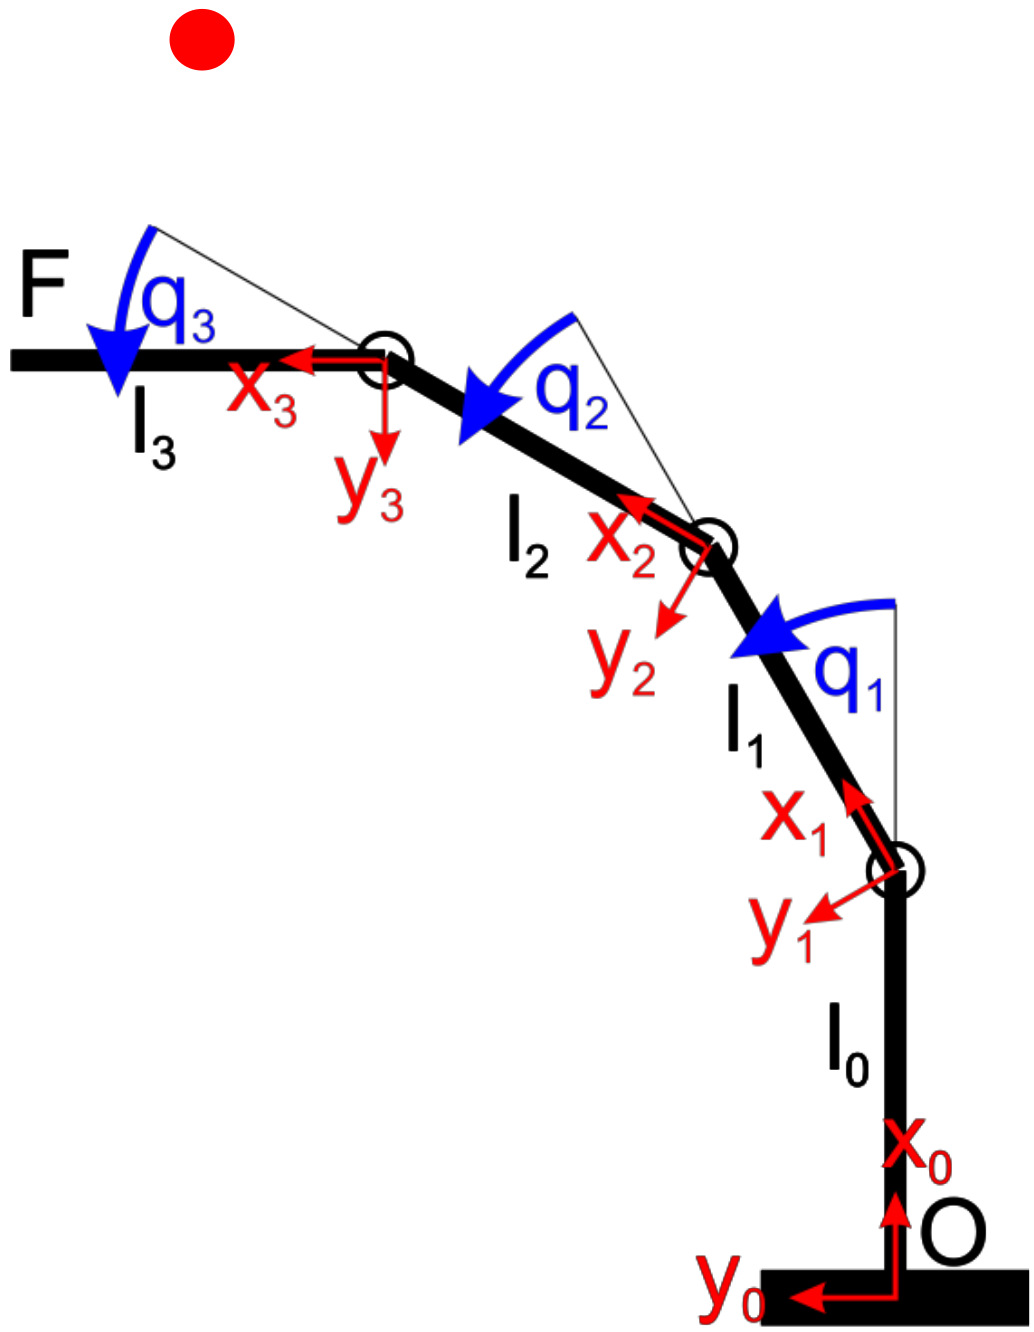
\includegraphics[width=\linewidth]{./Figures/03_InverseKinematrics.png}
\end{minipage}

\subsection{Inverse Differential Kinematics}
\begin{itemize}
    \item Given desired endeffector velocity $\dot r_{F} = J_P \dot q = r^\text{goal}_F$, determine generalized velocity $q = J^+_P \dot r^\text{goal}_F$
\end{itemize}

\subsection{Redundancy and Singularity}
\begin{itemize}
    \ides{Redundancy:} Jacobian is column-rank deficient
        \begin{itemize}
            \item Pseudo inverse minimizes $\norm{\dot q}_2$
            \item Can have multiple solutions $\dot q = J^+ \dot r^\text{goal} + \underbrace{(I - J^+ J)}_{N} \dot q_0$
            \item $q_0$ is chosen solution
        \end{itemize}
    \ides{Singularity:} Jacobian is row-rand deficient
        \begin{itemize}
            \item Pseude inverse minimizes error $\norm{\dot r^\text{goal} - \dot r}_2$
        \end{itemize}
\end{itemize}

\subsection{Mobile Robot Kinematics}
\begin{itemize}
    \ides{Legged Robot:} Quadropad
        \begin{itemize}
            \item $q =
                \begin{bmatrix}
                    q_B\\
                    q_r
                \end{bmatrix}
                \begin{matrix}
                    \text{Un-actuated base}\\
                    \text{Actuated joints}
                \end{matrix}$
            \ides{Contact Constraint:} $\dot r_F = J_F \dot q = 0 \Rightarrow \dot q = \cancel{J^+_F \dot r_F}^{=0} + N_F \dot q_0$
            \ides{Body Move:} $\dot r_B = J_B \dot q = J_B N_F \dot q_0$
        \item $\dot q = \cancel{J^+_F \dot r_F}^{=0} + N_F \dot q_0 = N_F(J_B N_F)^+ \dot r_B$
        \end{itemize}
    \ides{Wheeled Robot:} Planar car
        \begin{itemize}
            \item $q =
                \begin{bmatrix}
                    x\\
                    \varphi
                \end{bmatrix}$
            \item Point on wheel: ${}_I r_{OP} =
                \begin{bmatrix}
                    x + r \sin(\varphi)\\
                    r + r \cos(\varphi)\\
                        0
                \end{bmatrix}$
            \item ${}_I J_P =
                \begin{bmatrix}
                    1 & r \cos(\varphi)\\
                    0 & -r \sin(\varphi)\\
                    0 & 0
                \end{bmatrix}$
        \ides{Contact Constraint:} $\left. {}_I \dot x_P \right|_{\varphi = \pi} = \left. {}_I J_P \right|_{\varphi = \pi} \dot q =
                    \begin{bmatrix}
                        1 & -r\\
                        0 & 0\\
                        0 & 0
                    \end{bmatrix}
                    \begin{bmatrix}
                        \dot x\\
                        \dot \varphi
                    \end{bmatrix} = 0$
            \ides{Rolling Constraint:} $\dot x - r \dot \varphi = 0$
        \end{itemize}
\end{itemize}

\subsection{Mobile Robots}
\begin{itemize}
    \ides{Holonomic:}
        \begin{itemize*}
            \item Can move instantaneously in any direction of its DoF
            \item Differential constraints are integrable
        \end{itemize*}
    \ides{Non-Holonomic:}
        \begin{itemize*}
            \item Cannot move instantaneously in any direction of its DoF
            \item Differential constraints are not integrable
        \end{itemize*}
    \ides{Differential Forward Kinematics:} Given set of actuator speeds, determine its corresponding velocity
    \ides{Differential Inverse Kinematics:} given a desired velocity, determine the corresponding actuator speeds
\end{itemize}

\subsubsection{Wheel Kinematic}
\begin{minipage}[b]{0.48\linewidth}
    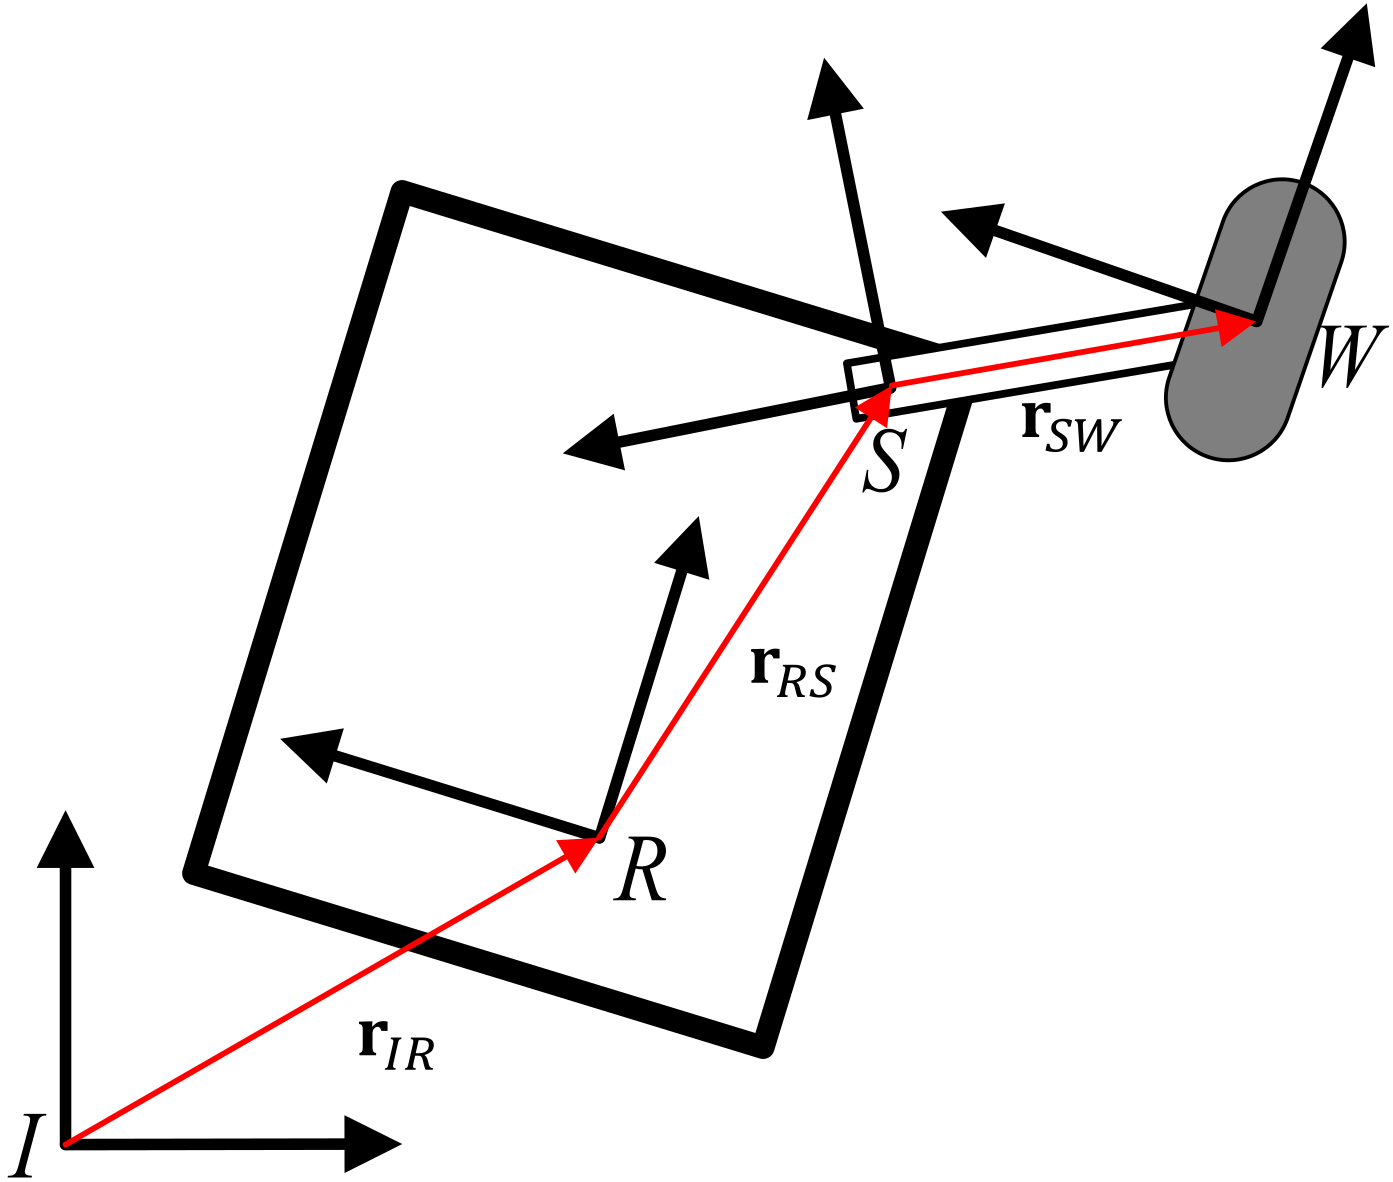
\includegraphics[width=\linewidth]{./Figures/03_WheelEquation.png}
\end{minipage}
\begin{minipage}[b]{0.48\linewidth}
    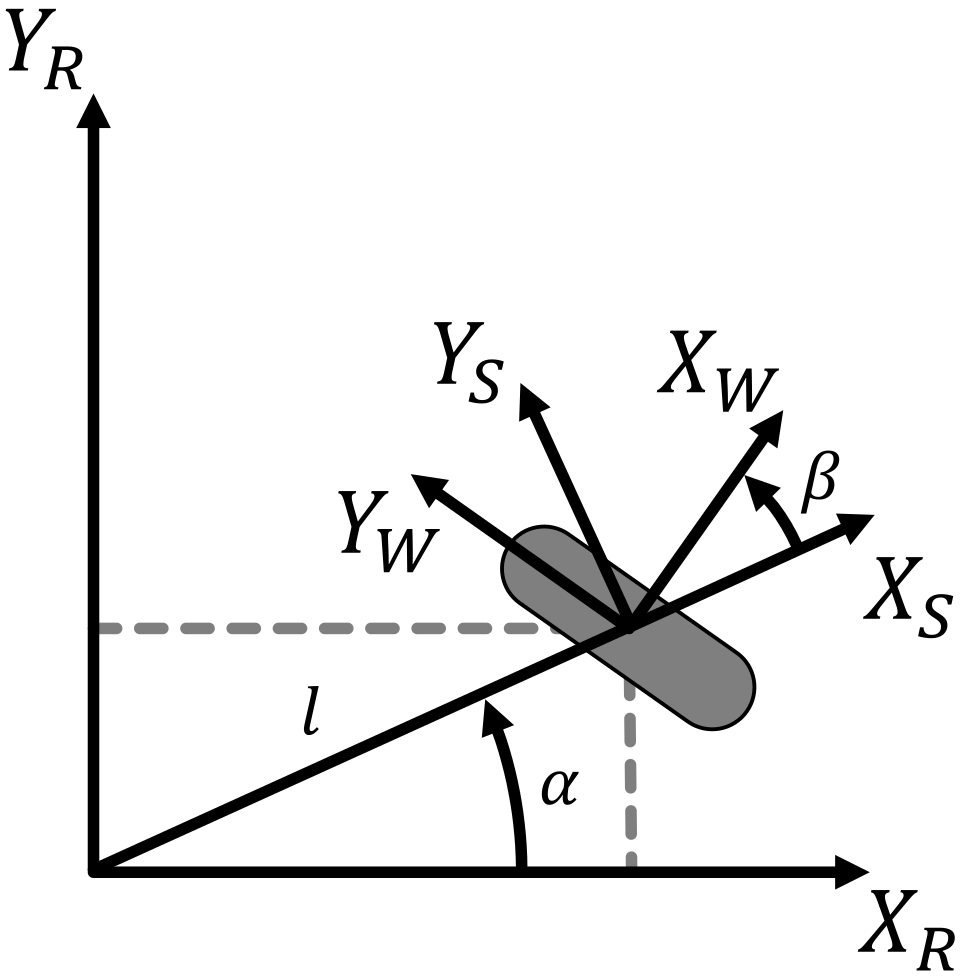
\includegraphics[width=\linewidth]{./Figures/03_StandardWheel.png}
\end{minipage}

\begin{itemize*}
    \item Robot state: $\xi_I = [x, y, \theta]^\transpose$
    \item $\dot \xi_I = [\dot x, \dot y, \dot \theta]^\transpose$
    \item $\dot \xi_R = R(\theta) \dot \xi_I$
    \item $R(\theta) = R^\transpose_z(\theta)$
\end{itemize*}
\begin{itemize}
    \item ${}_W v_{IW} =
        \begin{bmatrix}
            0\\
            -r \dot \varphi\\
            0
        \end{bmatrix}
        \begin{matrix}
            \text{no-sliding constraint}\\
            \text{rolling constraint}\\
            \text{planar assumption}
        \end{matrix}$
    \ides{Rolling Constraint:} $J_1(\beta_s) R(\theta) \dot \xi_I - \dot \varphi r = 0$
    \ides{No-Sliding Constraint:} $C_1(\beta_s) R(\theta) \dot \xi_I = 0$
    \ides{General Wheel Equation:} $v_{IW} = v_{IR} + \omega_{IR} \times r_{RS} + \omega_{IR} \times r_{SW} + \omega_{RS} \times r_{SW}$
    \ides{Standard (Steered \& Fixes) Wheel:} $r_{SW} = 0$
        \begin{itemize}
            \ides{Wheel Equation:} $v_{IW} = v_{IR} + \omega_{IR} \times r_{RS}$
                \begin{itemize}
                    \item ${}_W v_{IR} = R(\alpha + \beta) R(\theta)[\dot x, \dot y, 0]^\transpose$
                    \item ${}_W \omega_{IR} \times {}_W r_{RS} = [l \dot \theta \sin(\beta), l \dot \theta \cos(\beta), 0]^\transpose$
                \end{itemize}
            \item $J_1(\beta_s) = [\sin(\alpha + \beta_s), -\cos(\alpha + \beta_s), -l \cos(\beta_s)]$
            \item $C_1(\beta_s) = [\cos(\alpha + \beta_s), \sin(\alpha + \beta_s), l \sin(\beta_s)]$
            \item If fixed, $J_1(\beta_s) = J_1, C_1(\beta_s) = C_1$
            \item Only wheel which imposes constraints
        \end{itemize}
    \ides{Castor Wheel:}
        \begin{itemize}
            \item $J_1(\beta_s)$ same as standard wheel
            \item $C_1(\beta_s) = [\cos(\alpha + \beta_s), \sin(\alpha + \beta_s), d + l \sin(\beta)]$
        \end{itemize}
    \ides{Swedish Wheel:}
        \begin{itemize}
            \item $J_1(\beta_s) = [\sin(\alpha + \beta_s + \gamma), -\cos(\alpha + \beta_s + \gamma), -l \cos(\beta_s + \gamma)]$
            \item $C_1(\beta_s) = [\cos(\alpha + \beta_s + \gamma), \sin(\alpha + \beta_s + \gamma), l \sin(\beta_s + \gamma)]$
        \end{itemize}
\end{itemize}

\subsubsection{Mobile Robot Kinematic}
\begin{itemize}
    \item $N = (N_f + N_s)$ wheeled robot
\end{itemize}
\begin{itemize*}
    \item $J_1(\beta_s) =
        \begin{bmatrix}
            J_{1f}\\
            J_{1S}(\beta_s)
        \end{bmatrix}$
    \item $C_1(\beta_s) =
        \begin{bmatrix}
            C_{1f}\\
            C_{1S}(\beta_s)
        \end{bmatrix}$
    \item $J_2 = \mathrm{diag}(r_1, \dots, r_N)$
    \item $\dot \varphi =
        \begin{bmatrix}
            \dot \varphi_f\\
            \dot \varphi_s
        \end{bmatrix}$
\end{itemize*}
\begin{itemize}
    \ides{Rolling Constraint:} $J_1(\beta_s) R(\theta) \dot \xi_I - J_2 \dot \varphi = 0$
    \ides{No-Sliding Constraint:} $C_1(\beta_s) R(\theta) \dot \xi_I = 0$
    \item $
        \underbrace{\begin{bmatrix}
            J_1(\beta_s)\\
            C_1(\beta_s)
        \end{bmatrix}}_{A} \underbrace{R(\theta) \dot \xi_I}_{\dot \xi_R} =
        \underbrace{\begin{bmatrix}
            J_2\\
            0
        \end{bmatrix}}_{B} \dot \varphi$
    \ides{Forward Kinematics:} $\dot \xi_R = (A^\transpose A)^{-1} A^\transpose B \dot \varphi = A^+ B \dot \varphi$
    \ides{Inverse Kinematics:} $\dot \varphi = (B^\transpose B)^{-1} B^\transpose A \dot \xi_R = B^+ A \dot \varphi$
    \ides{Differential Drive:}
        \begin{itemize*}
            \item $\alpha_r = -\pi / 2$
            \item $\beta_r = \pi$
            \item $l_r = b$
            \item $r_r = r$
            \item $\alpha_r = \pi / 2$
            \item $\beta_r = 0$
            \item $l_l = -b$
            \item $r_l = r$
            \item $
                \begin{bmatrix}
                    \dot x\\
                    \dot y\\
                    \dot \theta
                \end{bmatrix}_R =
                \begin{bmatrix}
                    r / 2 & r / 2\\
                    0 & 0\\
                    r / 2b & -r / 2b
                \end{bmatrix}
                \begin{bmatrix}
                    \dot \varphi_r\\
                    \dot \varphi_l
                \end{bmatrix}$
            \item $
                \begin{bmatrix}
                    \dot \varphi_r\\
                    \dot \varphi_l
                \end{bmatrix} =
                \begin{bmatrix}
                    1 / r & 0 & b / r\\
                    1 / r & 0 & -b / r
                \end{bmatrix}
                \begin{bmatrix}
                    \dot x\\
                    \dot y\\
                    \dot \theta
                \end{bmatrix}_R$
        \end{itemize*}
\end{itemize}

\subsubsection{Maneuverability}
\begin{itemize}
    \ides{Degree of Maneuverability $\mathbf{\delta_M}$} $= \delta_m + \delta_s$
    \ides{Degree of Mobility $\mathbf{\delta_m}$:} $= \mathrm{dim} \; N(C_1(\beta_S)) = 3 - \mathrm{rank}(C_1(\beta_s))$
        \begin{itemize*}
            \item $0 \le \delta_m \le 3$
            \item $\delta_m = 0 \Rightarrow N_f = N_s = 0$
            \item $\delta_m = 3 \Rightarrow$ motion not possible
        \end{itemize*}
    \ides{Degree of Steerability $\mathbf{\delta_s}$:} $= \mathrm{rank}(C_{1s}(\beta_s))$
        \begin{itemize*}
            \item $0 \le \delta_s \le 2$
            \item $\delta_s = 0 \Rightarrow N_s = 0$
            \item $\delta_s = 1 \Rightarrow N_s \ge 1$
            \item $\delta_s = 2 \Rightarrow N_f = 0$
        \end{itemize*}
    \ides{Examples:}\\
\end{itemize}
{\footnotesize
    \begin{tabular}{l | l | l | l | l | l | l | l | l | l}
        & \rotatebox{90}{Omnidirectional}
        & \rotatebox{90}{Differential}
        & \rotatebox{90}{Omni-Steer}
        & \rotatebox{90}{Tricyle}
        & \rotatebox{90}{Two-Steer}
        & \rotatebox{90}{Ackerman Steer}
        & \rotatebox{90}{Bicycle}
        & \rotatebox{90}{Synchro Drive}
        & \rotatebox{90}{Onmi Drive}\\\hline
        $\delta_M$ & 3 & 2 & 3 & 2 & 3 & 2 & 2 & 2 & 3\\
        $\delta_m$ & 3 & 2 & 2 & 1 & 1 & 1 & 1 & 1 & 3\\
        $\delta_s$ & 0 & 0 & 1 & 1 & 2 & 1 & 1 & 1 & 0
    \end{tabular}
}

\subsection{Motion Control - Feedback Control}
    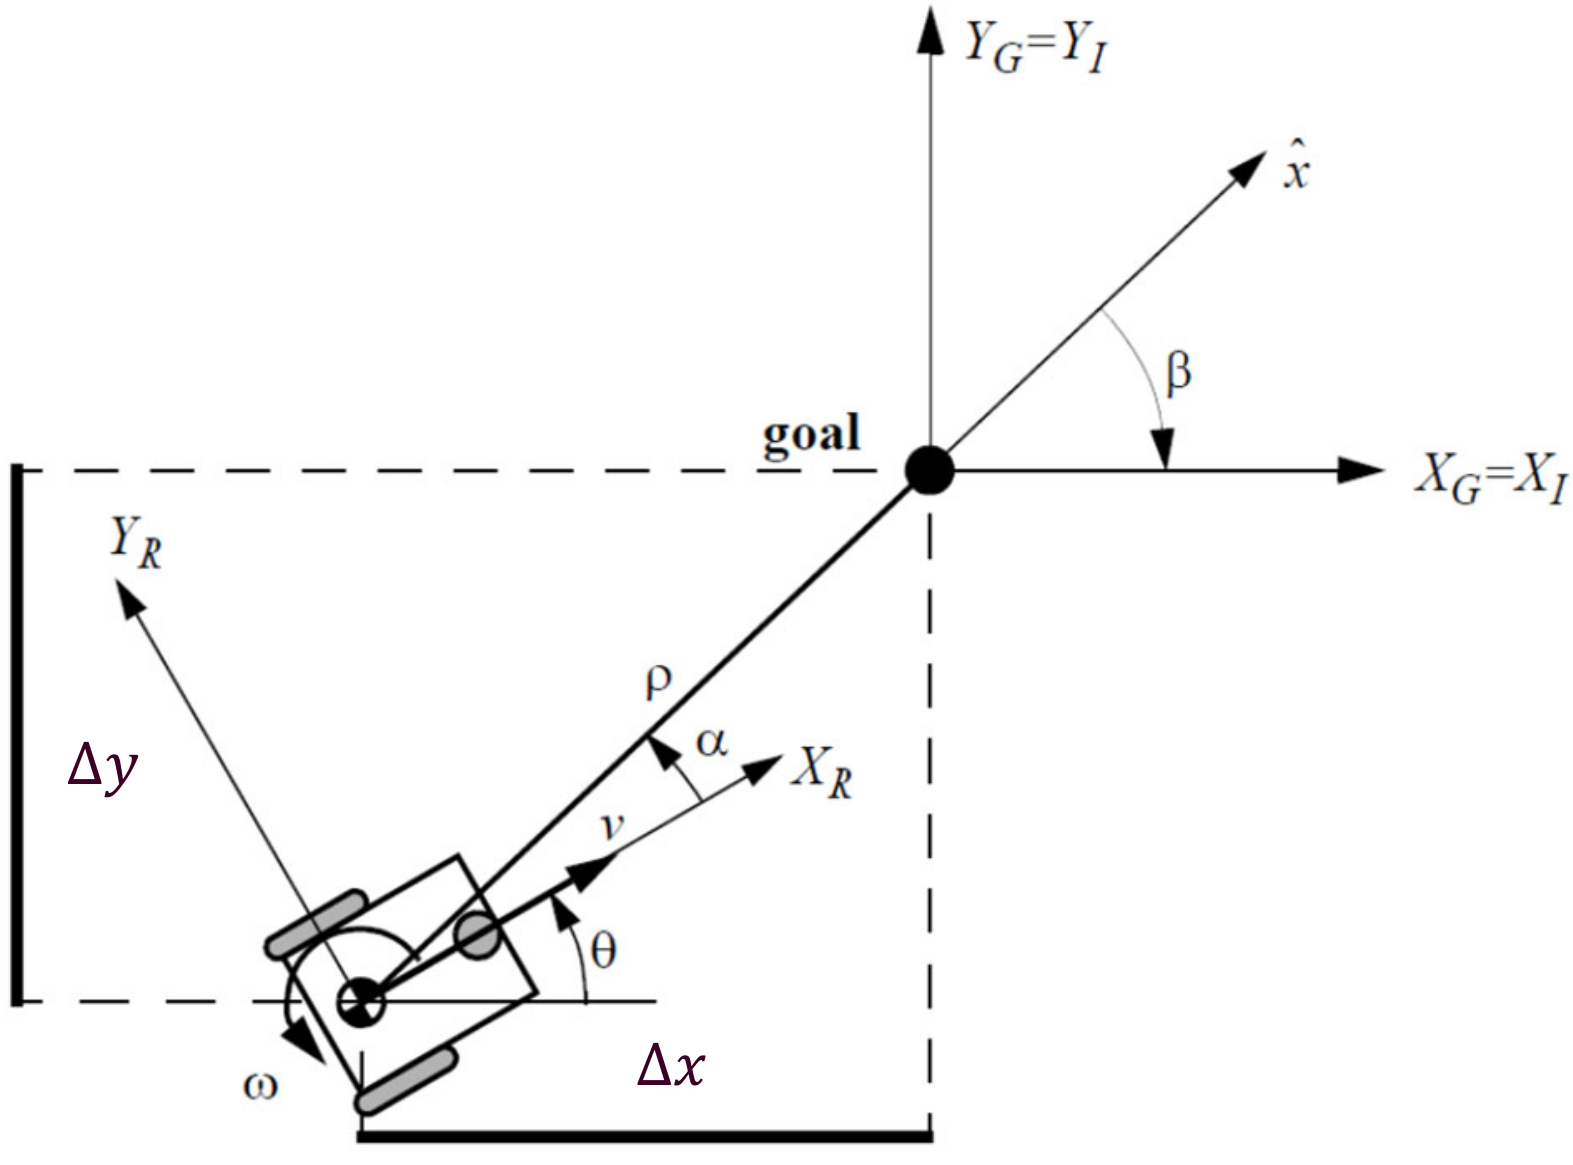
\includegraphics[width=\linewidth]{./Figures/03_MotionControl.png}
\begin{itemize}
    \item Drive robot from ${}_I[x, y, \delta]$ to ${}_I[0, 0, 0]$
    \ides{Error:} $e = [x, y, \delta]^\transpose$
    \item Get control inputs as $
        \begin{bmatrix}
            v(t)\\
            \omega(t)
        \end{bmatrix} = K \cdot e = K
        \begin{bmatrix}
            x\\
            y\\
            \theta
        \end{bmatrix}$
    \item Find $K$ such that $lim_{t \to \infty} e(t) = 0
        \begin{bmatrix}
            \dot x\\
            \dot y\\
            \dot \theta
        \end{bmatrix}_I =
        \begin{bmatrix}
            \cos \theta & 0\\
            \sin \theta & 0\\
            0 & 1
        \end{bmatrix}
        \begin{bmatrix}
            v\\
            \omega
        \end{bmatrix}$
    \item Polar Coordinate Transformation:
        \begin{itemize*}
            \item $\rho = \sqrt{\bigtriangleup x^2 + \bigtriangleup y ^2}$
            \item $\alpha = -\theta + \mathrm{atan2}(\bigtriangleup y, \bigtriangleup x)$
            \item $\beta = -\theta - \alpha$
            \item $\alpha, \beta \in [-\pi, \pi]$
        \end{itemize*}
    \item If $\alpha \in (-\frac{\pi}{2}, \frac{\pi}{2})$: $
        \begin{bmatrix}
            \dot \rho\\
            \dot \alpha\\
            \dot \beta
        \end{bmatrix} =
        \begin{bmatrix}
            -\cos \alpha & 0\\
            \frac{\sin \alpha}{\rho} & -1\\
            -\frac{\sin \alpha}{\rho} & 0
        \end{bmatrix}
        \begin{bmatrix}
            v\\
            \omega
        \end{bmatrix}$
    \item Otherwise: $
        \begin{bmatrix}
            \dot \rho\\
            \dot \alpha\\
            \dot \beta
        \end{bmatrix} =
        \begin{bmatrix}
            \cos \alpha & 0\\
            -\frac{\sin \alpha}{\rho} & 1\\
            \frac{\sin \alpha}{\rho} & 0
        \end{bmatrix}
        \begin{bmatrix}
            v\\
            \omega
        \end{bmatrix}$
    \item Control Law: $
        \begin{bmatrix}
            \dot \rho\\
            \dot \alpha\\
            \dot \beta
        \end{bmatrix} =
        \begin{bmatrix}
            -k_\rho \rho \cos(\alpha)\\
            k_\rho \sin(\alpha - k_\alpha \alpha - k_\beta \beta)\\
            -k_\rho \sin(\alpha)
        \end{bmatrix}$
    \item $v$ has a constant sign for one run
    \item Stable if $k_\rho > 0, k_\beta < 0, k_\alpha - k_\rho > 0$
\end{itemize}
